%\documentclass[showpacs,preprintnumbers,amsmath,amssymb,superscriptaddress,aip]{revtex4-1}
\documentclass[letter,scriptaddress,twocolumn, prl,showkeys]{revtex4}
\usepackage{graphicx}
%\usepackage{amssymb}
%\setlength{\parindent}{0in}

% General Latex  --------------------------------------------------
\def\beq{\begin{equation}}
\def\eeq{\end{equation}}
\def\beqar{\begin{eqnarray}}
\def\eeqar{\end{eqnarray}}
\def\nn{\nonumber}
\def\ol{\overline}
\def\para{\parallel}

% Operators  ------------------------------------------------------
\newcommand{\diff}[2]{\frac{d#1}{d#2}}
\newcommand{\diffs}[2]{\frac{d^2#1}{d#2^2}}
\newcommand{\pdiff}[2]{\frac{\partial#1}{\partial#2}}
\newcommand{\pdiffs}[2]{\frac{\partial^2#1}{\partial#2^2}}
\newcommand{\pdiffxy}[3]{\frac{\partial^2#1}{\partial#2 \partial#3}}
\newcommand{\pdt}{\partial_t}
\newcommand{\pdr}{\partial_r}
\newcommand{\pdth}{\partial_\theta}
\newcommand{\pdrr}{\partial^2_r}

\newcommand{\enum}[2]{{#1}\times10^{#2}} % 4.2x10^{3} = \enum{4.2}{3}

\newcommand{\vect}[1]{{\bf #1}}
%\newcommand{\vect}{\overrightarrow}
%\newcommand{\vect}{\vec}
\def\div{\nabla\cdot}
\def\grad{\nabla}
\def\curl{\nabla\times}
\newcommand{\gradpar}{\grad_\parallel}
\newcommand{\gradperp}{\grad_\perp}
\newcommand{\gradr}{\grad_r}
\newcommand{\defeq}{\ensuremath{\stackrel{\text{\tiny def}}{=}}}

\newcommand{\savg}[1]{\left<{#1}\right>}
\newcommand{\vavg}[1]{\left<{#1}\right>_V}
\newcommand{\thavg}[1]{\left<{#1}\right>_\theta}

% Variable names  -------------------------------------------------
\newcommand{\vpar} {v_\parallel}
\newcommand{\Apar} {A_\parallel}
\newcommand{\jpar} {j_\parallel}
\newcommand{\kpar} {k_\parallel}
\newcommand{\kperp} {k_\perp }
\newcommand{\vperp} {v_\perp }
\newcommand{\kthe}{k_\theta}

\newcommand{\Evec}{\ensuremath{\boldsymbol{{\rm E}}}}
\newcommand{\Bvec}{\ensuremath{\boldsymbol{{\rm B}}}}
\newcommand{\Jvec}{\ensuremath{\boldsymbol{{\rm J}}}}
\newcommand{\Fvec}{\ensuremath{\boldsymbol{{\rm F}}}}
\newcommand{\fvec}{\ensuremath{\boldsymbol{{\rm f}}}}
\newcommand{\vE}{\ensuremath{\boldsymbol{{\rm v}_{E}}}}
\newcommand{\bo}{\ensuremath{\boldsymbol{{\rm b}_0}}}
\newcommand{\bvec}{\ensuremath{\boldsymbol{{\rm b}}}}
\newcommand{\xvec}{\ensuremath{\boldsymbol{{\rm x}}}}
\newcommand{\yvec}{\ensuremath{\boldsymbol{{\rm y}}}}
\newcommand{\zvec}{\ensuremath{\boldsymbol{{\rm z}}}}
\newcommand{\vvec}{\ensuremath{\boldsymbol{{\rm v}}}}
\newcommand{\jvec}{\ensuremath{\boldsymbol{{\rm j}}}}

\newcommand{\bxgp}{\bvec\times\gradperp}

\newcommand{\vve}{\ensuremath{\boldsymbol{{\rm v}}_{e}}}
\newcommand{\vvi}{\ensuremath{\boldsymbol{{\rm v}}_{i}}}
\newcommand{\vpe}{v_{\parallel e}}
\newcommand{\vpi}{v_{\parallel i}}
\newcommand{\vvE}{\ensuremath{\boldsymbol{{\rm v}}_{E}}}
\newcommand{\vvD}{\ensuremath{\boldsymbol{{\rm v}}_{D}}}

\newcommand{\nuei}{\nu_{ei}}
\newcommand{\nuii}{\nu_{ii}}
\newcommand{\nue}{\nu_{e}}
\newcommand{\nuen}{\nu_{en}}
\newcommand{\nuin}{\nu_{in}}
\newcommand{\kpe}{\kappa_{\parallel e}}

\newcommand{\rs}{\rho_{s}}
\newcommand{\ri}{\rho_{i}}
\newcommand{\wci}{\Omega_{i}}
\newcommand{\wcix}{\Omega_{ix}}
\newcommand{\wce}{\Omega_{e}}
\newcommand{\tomega}{\tilde\omega}
\newcommand{\Isat}{I_{\rm sat}}
\newcommand{\fmie}{\frac{m_i}{m_e}}
\newcommand{\fmei}{\frac{m_e}{m_i}}


% Often used dimensions
\newcommand{\cm}{\rm cm}
\newcommand{\mm}{\rm mm}
\newcommand{\cmn}{{\rm cm}^{-3}}
\newcommand{\mn}{{\rm m}^{-3}}
\newcommand{\eV}{\rm eV}
\newcommand{\G}{\rm G}
\newcommand{\T}{\rm T}



\begin{document}

\title{}

\author{B. Friedman}
\email{friedman@physics.ucla.edu}

\author{T.A. Carter}

\affiliation{Department of Physics and Astronomy, University of California, Los Angeles, California 90095-1547, USA}



\begin{abstract}

\end{abstract}

\maketitle

\section{Introduction}

Normal mode analysis -- the calculation of eigenvalues and eigenvectors of a linearized dynamical system -- has been used to solve many problems over the years.
Despite its wide-ranging success, it has failed in important instances, particularly in predicting the onset of subcritical turbulence in hydrodynamic flows. 
The reason for this failure was explained in the early 1990's when Trefethen and others attributed the pitfalls of normal mode analysis to the non-normality of linear operators of
dynamical systems~\cite{trefethen1993,schmid2007}. A non-normal operator has 
eigenvectors that are not orthogonal to one another. One consequence of eigenvector nonorthogonality is that even when all eigenvectors decay exponentially under linear evolution, 
superpositions of eigenvectors can grow, albeit transiently.
In other words, certain fluctuations of the laminar state can access free energy from background gradients even though normal mode fluctuations cannot.
When combined with nonlinear effects, this allows for sustained subcritical turbulence.
Such behavior is obscured by traditional normal mode analysis, which only effectively describes the long time asymptotic behavior of fluctuations under  
action of the linear operator. Transient growth, which can dominate turbulent evolution, can be discovered only through non-modal calculations.

Non-modal analysis has been embraced by the hydrodynamics community over the past two decades in the attempt to explain and predict subcritical turbulence. But the plasma community
generally relies on normal mode analysis to inform turbulent predictions and observations, with a few exceptions~\cite{camargo1998,camporeale2010,schekochihin2012}. 
Furthermore, non-modal treatments have generally been explanatory rather than predictive and have centered around the transition to turbulence in subcritical systems rather 
than on properties of fully-developed turbulence.
This paper takes up the task of developing an approach to understand turbulent properties using only non-modal linear calculations with the goal of 
ultimately making quantitative predictions.  Our approach is to calculate an average growth rate of turbulent fluctuations due to linear processes, specifically due to transient growth.  We model the
turbulent steady state as a series of processes:  (1) the turbulence starts as a spatially random state, (2) linear transient growth deterministically amplifies the turbulent energy (or
decrease it in wavenumber ranges where linear damping dominates), (3) nonlinear transfer sets in at a specified timescale, terminating the
transient growth process and re-randomizing the turbulent state (at which point the cycle repeats).    Optimally, the timescale for the final step would be the
nonlinear decorrelation time of the turbulent system, but in order to enable predictive capability, we employ critical balance
arguments to use a characteristic \emph{linear} time. Since there is no obvious single linear time scale, we test several and compare the results to determine which works best.
The procedure ultimately produces a growth rate that can be used
to predict turbulent properties such as saturation levels and transport rates through mixing length arguments.

\section{Non-Normality of the Hasegawa-Wakatani Model}

Before employing the non-modal technique, we explore the effect of non-normality in the well-known and well-analyzed Hasegawa-Wakatani (HW) model~\cite{hasegawa1983}. 
We consider both the original 2D and the extended 3D~\cite{biskamp1995} versions of the model in a straight, unsheared magnetic field. 
The HW model consists of two equations for the density $n$ and the electrostatic potential $\phi$. The 3D version of the model is

\beqar
\label{n_eq}
\pdiff{n}{t} = - {\mathbf v_E} \cdot \grad n - \kappa \pdiff{\phi}{y} + \xi \gradpar^2 (n - \phi) - D \gradperp^4 n, \\
\label{phi_eq}
\pdiff{\gradperp^2 \phi}{t} = - {\mathbf v_E} \cdot \grad (\gradperp^2 \phi) + \xi \gradpar^2 (n - \phi) - D \gradperp^6 \phi
\eeqar
The normalizations are $\phi \to e \phi/T_e, n \to n/n_0, \grad \to \rho_s \grad , x,y,z \to x,y,z/\rho_s, t \to \omega_{ci} t $. Additionally,
$\mathbf{v_E} = \mathbf{b} \times \grad \phi$, $\xi = 4 \pi \omega_{ce}/\nu_{ei}$, 
and $\kappa = \rho_s/L_n$, where $L_n$ is the density scale length. The terms $D \gradperp^4 n$ and $D \gradperp^6 \phi$ are artificial hyper-diffusion and hyper-viscosity used to dissipate
energy on small scales. We set $D \to 10^{-5}$ except when otherwise indicated.
We associate the direction along $\mathbf{B}$ as the parallel or $z$ direction. The direction perpendicular $\mathbf{B}$ that
points opposite the density gradient is defined as the $x$ direction, and the $y$ direction is taken perpendicular to both of these. 
In the analysis and numerical simulations, which we perform with the BOUT++ code~\cite{dudson2009}, we use periodic boundary conditions in
the $y$ and $z$ directions with zero-value boundaries in the $x$ direction. For the 2D version of the model, we replace $-\xi \gradpar^2$ by 
$\alpha = k_z^2 \xi = 4 \pi k_z^2 \rho_s^2 \omega_{ce} /\nu_{ei}$, which is commonly known as the adiabaticity parameter~\cite{camargo1995,camargo1998}.

The degree of non-normality of the linear operator in the HW model is largely a function of the adiabaticity parameter~\cite{camargo1998}, or in the 3D case, of $\xi \gradpar^2$. 
Note that a matrix is normal if it commutes with its adjoint: $\mathbf{D} \mathbf{D}^\dagger = \mathbf{D}^\dagger \mathbf{D}$ for $\mathbf{D}$ normal. 
The HW model has a normal linear operator in the limit of $\alpha, \xi \gradpar^2 \to \infty$. 
To see this, we first transform the linear operator into a linear matrix by using a Fourier decomposition. Because we use a zero-value boundary condition in the $x$ direction, the
Fourier decomposition takes the form:

\beq
\label{fourier_form}
f_k = \int_0^{L_x,L_y,L_z} f(\mathbf{r}) \ {\rm sin} \left( k_x x \right) e^{i k_y y + i k_z z} d\mathbf{r}
\eeq
where $k_x = \pi l/L_x, k_y = 2 \pi m/L_y, {\rm and } \ k_z = 2 \pi n/L_z$ with $l, m, {\rm and } \ n$ integers.
The result for the 3D model is an equation for each mode $k = (k_x,k_y,k_z)$:

\beqar
\label{fourier_eqn}
\frac{\partial}{\partial t} \left( \begin{array}{cc} n_k \\ \phi_k \end{array} \right) = \mathbf{A}_k \left( \begin{array}{cc} n_k \\ \phi_k \end{array} \right) + \mathbf{N}_k \left( \begin{array}{cc} n_k \\ \phi_k \end{array} \right), \\ \nonumber \\
\mathbf{A}_k = \left( \begin{array}{cc} -\xi k_z^2 - D k_\perp^4 & -i \kappa k_y + \xi k_z^2 \\  \xi \frac{k_z^2}{k_\perp^2} & - \xi \frac{k_z^2}{k_\perp^2} - D k_\perp^4\end{array} \right)
\eeqar
with $\mathbf{A}_k$ being the linear coupling matrix and $\mathbf{N}_k$ the nonlinear matrix, which we don't write explicitly. 
Now in assessing the degree of normality of the HW model, we are not interested in the normality of $\mathbf{A}_k$ itself. 
Rather, we are interested in the energetically-weighted version of this matrix~\cite{camargo1998,schmid2007,camporeale2010}. Since the energy in a given Fourier mode is

\beq
\label{en_def}
E_k =  \frac{1}{2} \left( |n_k|^2 + k_\perp^2 |\phi_k|^2 \right).
\eeq
we rewrite Eq.~\ref{fourier_eqn} as

\beqar
\label{fourier_en_eqn}
\frac{\partial}{\partial t} \left( \begin{array}{cc} n_k \\ k_\perp \phi_k \end{array} \right) = \mathbf{B}_k \left( \begin{array}{cc} n_k \\ k_\perp \phi_k \end{array} \right) + \mathbf{N}_k \left( \begin{array}{cc} n_k \\ k_\perp \phi_k \end{array} \right), \\ \nonumber \\
\mathbf{B}_k = \left( \begin{array}{cc} -\xi k_z^2 - D k_\perp^4 & -i \kappa \frac{k_y}{k_\perp} + \xi \frac{k_z^2}{k_\perp} \\  \xi \frac{k_z^2}{k_\perp} & - \xi \frac{k_z^2}{k_\perp^2} - D k_\perp^4\end{array} \right)
\eeqar
Since the square $L_2$-norm of the new state vector $\frac{1}{\sqrt{2}} \left( \begin{array}{cc} n_k \\ k_\perp \phi_k \end{array} \right)$ gives the energy contained in the mode $k$,
$\mathbf{B}_k$ is the energetically-weighted matrix of interest. In the limit of large $\xi k_z^2$ as long as $k_\perp$ is also not too large:

\beq
\label{B_norm_limit}
\displaystyle\lim_{\xi k_z^2 \to \infty} \mathbf{B}_k = \left( \begin{array}{cc} -\xi k_z^2 & \xi \frac{k_z^2}{k_\perp} \\  \xi \frac{k_z^2}{k_\perp} & - \xi \frac{k_z^2}{k_\perp^2} \end{array} \right)
\eeq
where it is easy to see that $\mathbf{B}_k$ is self-adjoint and therefore normal. In the opposite limit:

\beq
\label{B_norm_limit0}
\displaystyle\lim_{\xi k_z^2 \to 0} \mathbf{B}_k = \left( \begin{array}{cc} - D k_\perp^4 & -i \kappa \frac{k_y}{k_\perp} \\ 0  & - D k_\perp^4\end{array} \right)
\eeq
in which case $\mathbf{B}_k$ is non-normal. In general, as the adiabaticity parameter is varied, the normality of $\mathbf{B}_k$ changes, but unfortunatley there is no absolute metric to quantify
the normality of a matrix or operator~\cite{trefethen2005}. In practice, however, what matters is not how non-normal $\mathbf{B}_k$ is, but how much transient energy growth is possible in the linear
system. The linear HW system is

\beq
\label{lin_HW}
\diff{u_k}{t} = \mathbf{B}_k u_k
\eeq
where $u_k = \left( \begin{array}{cc} n_k \\ k_\perp \phi_k \end{array} \right)$. The solution to this $u_k(t) = e^{\mathbf{B}_k t} u(0)$ where the exponential of the matrix is defined in terms of
its Taylor expansion. The solution is dependent on the initial condition $u(0)$. The energy growth as a function of time is

\beq
\label{Gt}
G_k(t) = \frac{||u(t)||^2}{||u(0)||^2} = \frac{||e^{\mathbf{B}_k t} u(0)||^2}{||u(0)||^2}
\eeq
where the operator $|| \cdot ||$ is the $L_2$-norm. Different initial conditions provide optimal energy growth at different times, but the upper envelope of all such optimal growth curves is given by
$G_{k,\rm{max}}(t) = ||e^{\mathbf{B}_k t}||^2$, which does not depend on the initial condition.
Moreover, $||e^{\mathbf{B}_k t}||^2 \ge e^{2 \gamma_{s,k} t}$, where $\gamma_{s,k}$ is the real part of
the fastest growing (or least damped) eigenmode of $\mathbf{B}_k$ (and of $\mathbf{A}_k$, since $\mathbf{B}_k$ is just a similarity transform of $\mathbf{A}_k$~\cite{camargo1998}). 
The equality holds when $\mathbf{B}_k$ is normal, meaning the normal case provides a lower bound to the maximal energy growth. 
Thus, non-normality in practice allows a system to undergo more energy growth than is dictated by the most unstable linear eigenmode. We show this in Fig.~\ref{max_en_growth} where we plot
$||e^{\mathbf{B}_k t}||^2$ for different values of $\alpha$ along with $e^{2 \gamma_{s,k} t}$, showing that non-modal growth is possible for small adiabaticity parameter $\alpha$. Furthermore,
the short time transient growth becomes larger as $\alpha$ becomes smaller.

\begin{figure}
\centerline{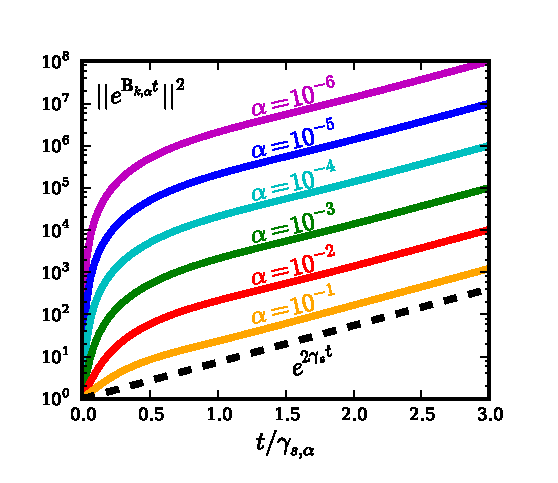
\includegraphics[width=0.45\textwidth]{max_en_growth}}
\caption{$G_{k,\alpha,\rm{max}}(t) = ||e^{\mathbf{B}_{k,\alpha} t}||^2$ for $k_x=0, k_y=1$ for different values of the 2D adiabaticity parameter 
$\alpha$ compared to the energy growth $e^{2 \gamma_{s,\alpha,k} t}$ of the least stable eigenmode of  $\mathbf{B}_{k,\alpha}$. 
The time axis is normalized to $\gamma_{s,\alpha}$, which is different for each of the curves. This normalization makes the $e^{2 \gamma_{s,\alpha,k} t}$ line the same for all $\alpha$. 
$||e^{\mathbf{B}_{k,\alpha} t}||^2$ displays large non-exponential growth at early times that increases with decreasing $\alpha$.}
\label{max_en_growth}
\end{figure}

One explanation for this behavior is that non-normal matrices or operators have non-orthogonal linear eigenvectors. For the HW model, each Fourier matrix $\mathbf{B}_k$ has two eigenvectors associated
with it. They are complex and take the form:

\beq
\label{lin_eigen_form}
\psi_{k,q} = \left( \begin{array}{cc} n_k \\ k_\perp \phi_k \end{array} \right)_q {\rm sin} \left( k_x x \right) e^{i k_y y + i k_z z} 
\eeq
where the subscript $q$ takes the values of $1$ and $2$, representing the two eigenvectors for each $k$. The two eigenvectors are different in that they have a different complex ratio $n_k/\phi_k$.
The two eigenvalues have different growth rates (the real part), but the same frequency, though with opposite sign.
As $\alpha \to 0$, the two eigenvectors become less orthogonal -- more parallel or anti-parallel to one another. When the eigenvectors are nearly anti-parallel and initialized with finite amplitude,
their superposition, which constitutes the total system at $k$, may linearly evolve so that the norm of the superposition grows faster than either individual eigenvector. A paradigmatic illustration
of this may be seen in a review by Schmid~\cite{schmid2007}.

\section{The Effect of Non-Normality on Turbulence}

Linear non-normality is important for the effect it has on turbulence. It is most often cited as the sufficient condition for turbulence in subcritical systems, 
but it can also impact systems that have unstable linear eigenmodes like the HW system. Since certain superpositions of the linear eigenmodes can inject energy faster than the most unstable linear
eigenmode, there is the possibility that the energy injection into the turbulence is faster and at different wavenumbers than that suggested by linear eigenmode analysis. 
To understand this concept and show that it occurs in the nonlinear HW model, we compare the fastest growing linear eigenmode growth rate $\gamma_{s,k}$ to the turbulent growth rate $\gamma_{t,k}$. 
First, however, we define the turbulent growth rate and show how to calcuate it for the HW model.
In order to find the turbulent growth rate for the HW model, we use a Fourier-decomposed energy dynamics analysis~\cite{camargo1995,friedman2012b,friedman2013}. 
To do this, we take Eqs.~\ref{n_eq} and~\ref{phi_eq} and substitute the following:

\beqar
\label{subs_fourier}
n = \sum_{k} n_k {\rm sin} \left( k_x x \right) e^{i k_y y + i k_z z} \\
\phi = \sum_{k} \phi_k {\rm sin} \left( k_x x \right) e^{i k_y y + i k_z z},
\eeqar
where again $k$ is shorthand for $(k_x,k_y,k_z)$.
Then, we multiply the resulting first equation by $n^*_{k'} {\rm sin} \left( k'_x x \right) e^{-i k'_y y - i k'_z z}$ and the second equation by 
$-\phi^*_{k'} {\rm sin} \left( k'_x x \right) e^{-i k'_y y - i k'_z z}$, take the volume integral and add the equations together. The result is

\beqar
\label{Explicit_En_eqn}
\frac{1}{2} \diff{}{t} \left( |n_k|^2 + k^2_\perp |\phi_k|^2 \right) = -i k_y \kappa \phi_k n^*_k - \xi k_z^2 |n_k - \phi_k|^2 \nonumber \\
- D k^4_\perp \left( |n_k|^2 + k^2_\perp |\phi_k|^2 \right) + \sum_{k'} T(k,k')
\eeqar
where, again, the energy $E_k$ is $\frac{1}{2} \left( |n_k|^2 + k^2_\perp |\phi_k|^2 \right)$, 
and the term $\sum_{k'} T(k,k')$ represents the nonlinear contribution (three-wave transfers between different $k$'s), 
which we do not write explicitly. This energy evolution equation may be written symbolically as

\beq
\label{dEdt_def}
\diff{E_k}{t} = \diff{E_{l,k}}{t} + \diff{E_{nl,k}}{t}
\eeq
where $\diff{E_{l,k}}{t}$ represents the terms that come from the linear terms in Eqs.~\ref{n_eq} and~\ref{phi_eq}. These are actually quadratic in the fluctuating
quantities $n_k$ and $\phi_k$ in Eq.~\ref{Explicit_En_eqn}. 
$\diff{E_{l,k}}{t}$ represents the injection of energy into the fluctuations from the free energy in the equilibrium gradients plus the dissipation from collisions and hyperdiffusion.
$\diff{E_{nl,k}}{t}$ represents $\sum_{k'} T(k,k')$ in  Eq.~\ref{Explicit_En_eqn} and comes from the nonlinear terms in 
Eqs.~\ref{n_eq} and~\ref{phi_eq}. The terms in $T(k.k')$ are triadic in the fluctuating quantities and
account for the energy exchange between fluctuations with different $k$. Furthermore, it is conservative: $\sum_{k} \diff{E_{nl,k}}{t} = \sum_{k,k'} T(k,k') = 0$.
Now, in quasi-steady state turbulence, the rate of net energy injection (or dissipation) into the fluctuations at each $k$ by the linear terms must be balanced by
the rate of energy removal (or deposition) from the nonlinear terms. This may be represented formally using growth rates:

\beqar
\label{steady_state}
\gamma_k \equiv  \displaystyle\lim_{T \to \infty} \frac{1}{T} \int_0^T \frac{dE_k/dt}{2 E_k} dt \nonumber \\
= \displaystyle\lim_{T \to \infty} \frac{{\rm{Log}}\left[ E_k(T)/E_k(0) \right]}{2 T} = 0
\eeqar
where the equality to zero clearly holds as long as the turbulence is in a steady or quasi-steady state.
From, Eqs.~\ref{dEdt_def} and~\ref{steady_state}, it follows that $ \gamma_k = \gamma_{l,k} + \gamma_{nl,k} = 0$.

We now associate the linear rate of energy injection into the fluctuations $\gamma_{l,k}$ as the turbulent growth rate $\gamma_{t,k}$ discussed above. 
It should be clear now that this growth rate is the turbulence equivalent to the linear eigenmode growth rate $\gamma_{s,k}$~\cite{friedman2012b,terry2006b}. 
Moreover, $\gamma_{l,k}$ is calculated from the spatial structures of the plasma state variables, so it is always well-defined, even in a turbulent plasma. In a linear simulation run for a
sufficiently long time where transients die away, the calculation of $\gamma_{l,k}$ gives exactly $\gamma_{s,k}$.

In a turbulent state, which can be considered a linear superposition of linear eigenvectors, $\gamma_{t,k} \le \gamma_{s,k}$ if the system is normal. Recall that in normal systems, the maximal
energy growth is given by the most unstable linear eigenmode. In other words, maximal growth is achieved when the most stable eigenmode has zero amplitude. When this subdominant eigenmode has finite
amplitude, the growth rate must be lowered. On the other hand, non-normal systems may grow faster than is dictated by the most unstable eigenmode when the subdominant eigenmode has finite amplitude. 
It is therefore possible for $\gamma_{t,k} \ge \gamma_{s,k}$ in non-normal systems. 

\begin{figure}
\centerline{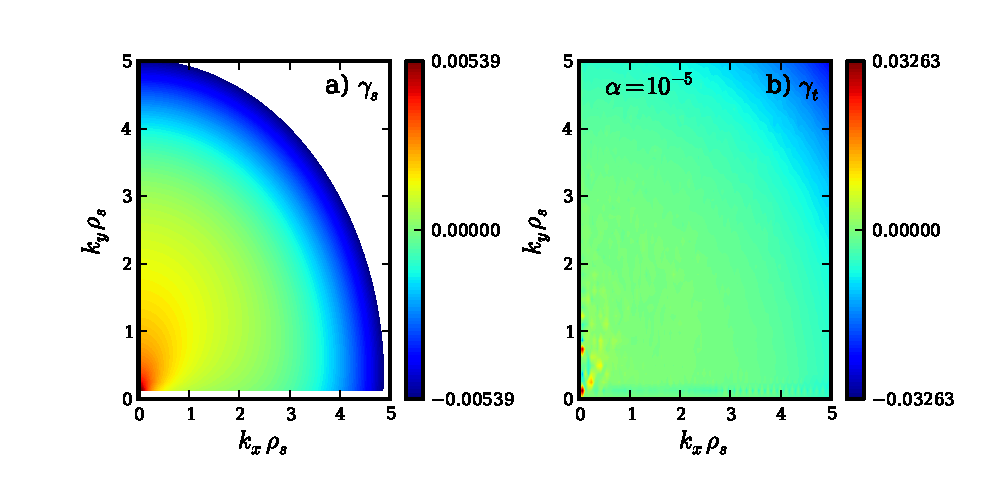
\includegraphics[width=0.55\textwidth]{alpha1e-5_gamma_s_t}}
\caption{a) The eigenmode growth rate spectrum $\gamma_{s,k}$ and b) the turbulent growth rate spectrum $\gamma_{t,k}$ for $\alpha = 10^{-5}$. Note the different scales.}
\label{alpha1e-5_gamma_s_t}
\end{figure}

\begin{figure}
\centerline{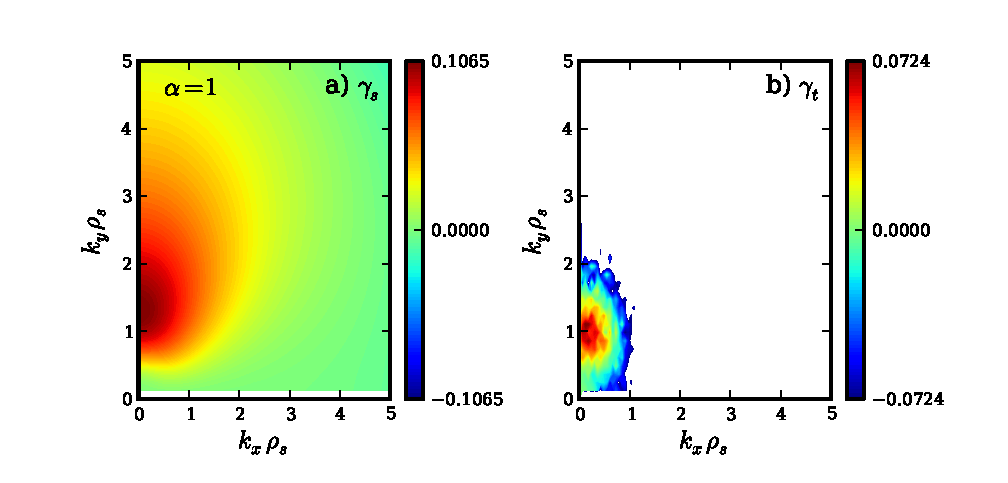
\includegraphics[width=0.55\textwidth]{alpha1_gamma_s_t}}
\caption{a) The eigenmode growth rate spectrum $\gamma_{s,k}$ and b) the turbulent growth rate spectrum $\gamma_{t,k}$ for $\alpha = 1$.}
\label{alpha1_gamma_s_t}
\end{figure}

For the 2D HW model, we show
$\gamma_{s,k}$ and $\gamma_{t,k}$ for two different values of $\alpha$. In Fig.~\ref{alpha1e-5_gamma_s_t}, we show these growth rate spectra for $\alpha = 10^{-5}$, for which the system is
highly non-normal, and in Fig.~\ref{alpha1_gamma_s_t} for $\alpha = 1$, for which the system is very close to being normal. Note the different scales used in all of the figures. In the highly
non-normal case, the turbulent growth rate is somewhat higher than the eigenmode growth rate for most values of $k_x,k_y$, and about 6 times higher where the spectrum peaks. For the more normal
case, in contrast, $\gamma_{t,k}$ is generally lower than $\gamma_{s,k}$, with the peak at less than a factor of 2 less, though the peaks are at slightly different values of $k_y$.

\begin{figure}
\centerline{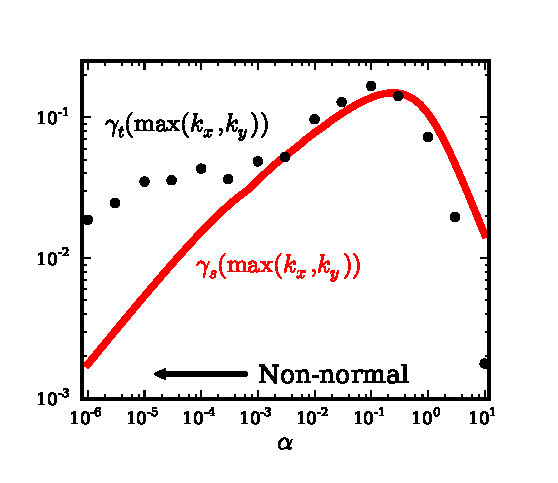
\includegraphics[width=0.4\textwidth]{gamma_max_vs_alpha}}
\caption{}
\label{gamma_max_vs_alpha}
\end{figure}

We show the peak values for $\gamma_{s,k}$ and $\gamma_{t,k}$ in Fig.~\ref{gamma_max_vs_alpha} as a function of $\alpha$. The peak values always occur in $k$-space
at the lowest $k_x$ available to our system, corresponding to half of a period of a sine wave. The value of $k_y$ that gives the highest growth rate migrates upward as $\alpha$ increases,
as is clear from Figs.~\ref{alpha1e-5_gamma_s_t} and~\ref{alpha1_gamma_s_t}. Furthermore, as expected, when $\alpha$ is small $\lesssim 10^{-3}$, $\gamma_{t,k} > \gamma_{s,k}$, with
$\gamma_{t,k} \gg \gamma_{s,k}$ as $\alpha \to 0$. Additionally, when $\alpha$ becomes larger and the system becomes more normal ($\gtrsim 10^{-1}$), $\gamma_{t,k} < \gamma_{s,k}$.
For both the normal and highly non-normal limits of the 2D HW model, $\gamma_{s,k}$ does a poor job of predicting $\gamma_{t,k}$ because $\gamma_{s,k}$ neglects the stable branch of the
dispersion relation -- the damped eigenmode. The importance of the stable eigenmode branch has started to gain acceptance in the plasma community, although it has generally been used to explain
turbulent saturation, as is the case for nearly normal systems~\cite{terry2006}. The increased turbulent excitation in the highly non-normal case, however, is not as well-known but it also
important.


\begin{figure}
\centerline{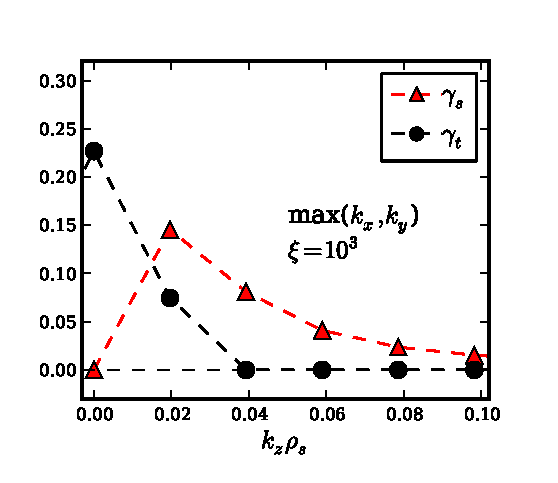
\includegraphics[width=0.4\textwidth]{gamma_max_vs_kz}}
\caption{}
\label{gamma_max_vs_kz}
\end{figure}

The nonlinear simulation reveals a fascinating property of the turbulence -- 
it is dominated by a nonlinear instability process despite being linearly unstable to drift waves~\cite{friedman2012b,friedman2013}.
The nonlinear instability, which was discovered by Drake et al.~\cite{drake1995}, works as follows: 
magnetic-field-aligned ($k_\para=0$) convective filaments transport density across the equilibrium density gradient, setting up $k_\para=0$ density filaments. 
These filaments are unstable to secondary drift waves, which grow on the periphery of the filaments. 
These drift waves, which have finite $k_\para$, nonlinearly couple to one another and generate new convective filaments.

Although the instability is called a nonlinear instability, the first part of the mechanism -- the transport of background density by the convective filaments -- is a linear one.
In fact, the other parts of the mechanism are driven by energetically conservative nonlinear interactions, 
meaning that the convective transport is the only step responsible for energy injection into the fluctuations.


This convective transport of density filaments is akin to the paradigmatic ``lift-up'' mechanism in hydrodynamic shear flows whereby streamwise vortices drive streamwise 
streaks~\cite{trefethen1993,krommes1999}.
Both are transient growth processes.

\section{Non-Modal Linear Technique of Turbulent Growth Rate}



We contend that the key to understanding and predicting turbulent properties through non-modal analysis is 
to successfully model the effect that the nonlinearities have on the transient linear processes. 
To this effect, we note that the advective nonlinearity in Eq.~\ref{fourier_en_eqn} has the form of the state vector divided by a time $\tau_{nl} \sim (v_E k_\perp)^{-1}$. This nonlinear
time scale is generally associated with the eddy turnover or decorrelation time. We therefore present a heuristic model of the nonlinearities 
as a randomizing force that acts on this characteristic nonlinear time scale. Again, this model is one in which 1) the turbulence begins as a random state, 
2) evolves linearly for a time $\tau_{nl}$, and 3) randomizes by nonlinear energy transfer, at which point the steps repeat.
In practice, we implement this model by starting with an ensemble of random initial conditions, which we evolve linearly for a time $\tau_{nl}$, 
and then take the time and ensemble averaged growth rate of these curves.
This procedure does not require actual linear simulations from an ensemble of random initial conditions. To see this, recall that the time evolution of the energy from an initial condition is

\beq
\label{E_t_from_u0}
E_k(t) = ||e^{\mathbf{B}_k t} u(0)||^2 = e^{\mathbf{B}_k t} u(0) u^{\dagger}(0) e^{\mathbf{B}_k^{\dagger}t}.
\eeq
If the $\mathbf{u}(0)$ in the ensemble are random with uncorrelated components and normalized to unity, it follows that~\cite{camargo1998}

\beq
\label{E_t_ensemble_avg}
\left< E_k(t)/E_k(0) \right>_{{\rm{ens}}} = \frac{1}{2} {\rm{tr}} \{ e^{\mathbf{B}_k t} e^{\mathbf{B}^{\dagger}t} \}.
\eeq
One point to note is that in global equation sets like ours -- where we discritize and use finite differences in the radial direction rather than a Fourier decomposition -- randomizing $\mathbf{u}(0)$
amounts to setting the initial $k_r$ spectrum to a step function that goes to zero at the Nyquist wavenumber. This means that $\left< E(t)/E(0) \right>_{{\rm{ens}}}$ may depend on $N_r$, so we must be careful in
choosing $N_r$ for this analysis. We choose $N_r$ such that the grid spacing equals $\rho_s$, the general Nyquist wavenumber of drift wave simulations~\cite{scott1992}.

Mathematically, our procedure is to calculate $\gamma_{\rm{n-m}}$ by the following formula:

\beq
\label{gamma_l_calc}
\gamma_{\rm{nm},k} = \frac{1}{\tau_{nl}} \int_0^{\tau_{nl}} \frac{\pdiff{E_k(t)}{t}}{2 E_k(t)} dt = \frac{1}{2 \tau_{nl}} {\rm{Log}} \left[ \frac{E_k(\tau_{nl})}{E_k(0)}\right]
\eeq
where $E(t)$ is the ensemble averaged energy calculated from Eq.~\ref{E_t_ensemble_avg}, and $E(0) = 1$ by our normalization.
In order to move toward predictive capability, we must estimate $\tau_{nl}$ with only knowledge of linear (modal or non-modal) information. 
We thus invoke the conjecture of \emph{critical balance}, which posits that the nonlinear time scale equals the linear time scale at all spatial scales~\cite{schekochihin2012}. This follows from 
the previously derived steady-state result: $\gamma_l = - \gamma_{nl}$. 

Now there are two linear time scales that we may choose to test. The first linear time is the linear eigenmode frequency, labeled
$\omega_s^{-1}$. However, $\omega_s = 0$ for $k_z=0$ linear eigenmodes, so we are forced to use $\omega_s$ at the lowest finite $k_z$ to get a meaningful time scale.

Second, we use the steady-state condition $\gamma_l = - \gamma_{nl}$ and the approximation $\tau_{nl} \sim 1/|\gamma_{nl}|$ to get $\tau_{nl} = 1/|\gamma_{\rm{n-m}}|$. 
Inserting this into Eq.~\ref{gamma_l_calc} gives

\beq
\label{fourth_gamma_cond}
 {\rm{Log}} \left[ E_k(1/\gamma_{\rm{nm}})\right] = \pm 2 \ \rightarrow E_k(1/\gamma_{\rm{nm}}) = e^{\pm 2}.
\eeq
In other words, we find the time at which $E_k(t)$ grows to the value of $e^2$ or decays to the value of $e^{-2}$, and then use this time to get $\gamma_{nm}$.

\begin{figure}
\centerline{\includegraphics[width=0.55\textwidth]{alpha1e-5_gamma_spec_compare}}
\caption{}
\label{alpha1e-5_gamma_spec_compare}
\end{figure}

\begin{figure}
\centerline{\includegraphics[width=0.55\textwidth]{alpha1_gamma_spec_compare}}
\caption{}
\label{alpha1_gamma_spec_compare}
\end{figure}

\begin{figure}
\centerline{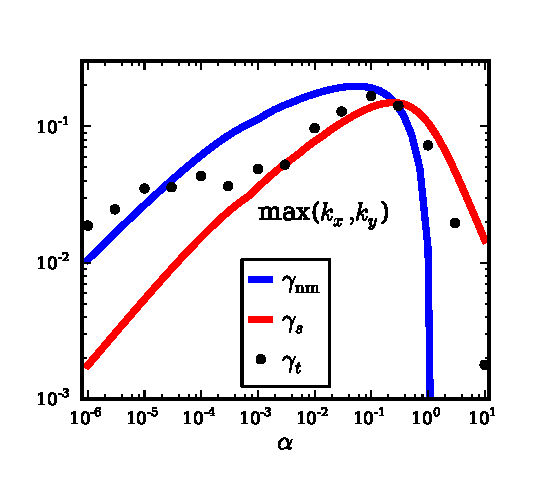
\includegraphics[width=0.55\textwidth]{gamma_max_with_nm}}
\caption{}
\label{gamma_max_with_nm}
\end{figure}

\begin{figure}
\centerline{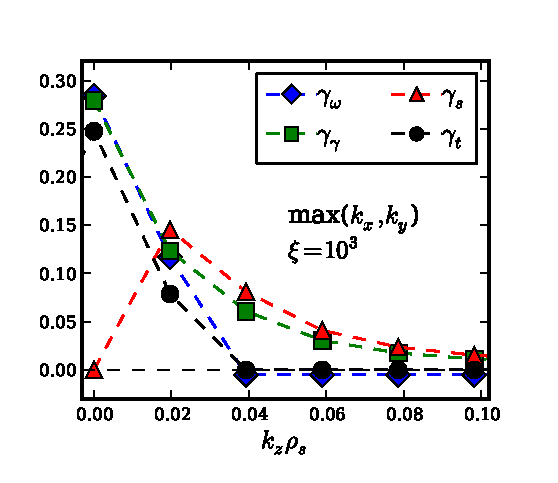
\includegraphics[width=0.4\textwidth]{gamma_max_vs_kz_with_nm}}
\caption{}
\label{gamma_max_vs_kz_with_nm}
\end{figure}


This work was supported by the National Science Foundation (Grant PHY-1202007)

%%%%%%%%%%%%%%%%%%%%%%%%%%%%%%%%%%%%%%%%%%%%%%%%%%%%%%%%%%%%%%%%%%%%%%%%%%%

%\bibliographystyle{phaip}
\bibliography{refs}

\end{document}
